\chapter{Interaction}
\label{sec:interaction}
In order to satisfactorily interact with the device, depending on physical, mental or social distractions, the user should be able to use the bracelet in different ways. Tasks that occur frequently should be completed in a very casual way, because tasks with low cognitive requirements are most likely still possible to execute successfully while the user is distracted. Rather infrequent tasks are allowed to demand more of the user's attention and cognitive capacity. If they occur rarely, the dissatisfaction of a failed task because of insufficient focus is not as grave as it would be if the task was a frequent one and if it would thus fail often.

As introduced in section \ref{sec:scenario}, the user should be able to turn the lights on or off with a minimum of engagement, so the task would still be possible while for example physical encumbrance hinders the user from performing more complex interactions. Also, the action should not require more effort than moving to the wall switch and pressing it. 

A similar amount of or only slightly increased complexity in interaction should be required for dimming the lights, because this is also a frequently used function in daily life. The analogy of turning a dimmer knob makes this interaction easy to associate with its function. Dimming should be performable while under some degree of distraction, for example while participating in a conversation. Since both hands and a focused rotational movement are needed, acceptable physical distractions quickly reach a tolerance limit.

More focus could be required for changing the color in a fuzzy way, according to the concept of \textit{mood} derived from color psychology, on a loose range from calming to stimulating. Since this function would probably not used very often, an interaction which requires a glance on the device to locate the proper spot for touching is considered reasonable. 

Changing the exact appearance of the light in terms of color, brightness and saturation however requires concentration and focus on the task, therefore the associated interaction with the bracelet can demand more of the user's engagement. Picking a certain template of presets in light color and setting is also a rather complex cognitive task that would happen infrequently, so associating it with a focused interaction seems appropriate.

\begin{table}
	\myfloatalign
	%$\left \Downarrow 
	\begin{tabularx}{.95\textwidth}{cc}
		\toprule
		\tableheadline{Task} & \tableheadline{Associated Interaction}\\ 
		\midrule
		switching on/off & covering touch area\\
		adjusting brightness & covering touch area, twisting the wrist\\
		fuzzy mood change & touch on two specific segments\\
		precise color change & combination of touch, slide, tap\\
		picking preset template & double tap and hand gesture\\
		\bottomrule
	\end{tabularx}
	%\right \downarrow $
	\caption[Tasks and associated interactions with the bracelet]{Tasks and associated interactions with the bracelet, in ascending complexity of the interaction and decreasing occurrence of the task}  \label{tab:interaction}
\end{table}

Table \ref{tab:interaction} shows how different interactions correspond to the described tasks. The focus in matching them lies on the required amount of attention needed to successfully complete the interaction as well as on the cognitive load a certain interaction entails. 

Since switching the lights on or off occurs rather frequently, a very simple action was associated with it. Covering the whole touch area of the bracelet for a few moments will trigger the on or off function of the device. When twisting the hand while covering said area, the light dims accordingly (cf. figures \ref{fig:onoff}, \ref{fig:dim}). 

More complex tasks have more intricate interactions associated with them, for changing the lighting \textit{mood} a precise touch on two neighboring segments of the touch surface is required. This demands either a precise knowledge of the bracelet's shape and the layout of its components, or a concentrated glance at the touch surface in order to choose the right segments. Figure \ref{fig:mood} depicts this interaction.

A precise adjustment of the light in terms of hue, saturation and brightness requires even more focus on the task, since not only the function itself requires some concentration, but also the execution of the associated action does (cf. figure \ref{fig:colorchange}). To activate this settings mode, a single segment needs to be pressed, then the three attributes are set by sliding along the touch surface and switching to the next one with a tap on the bracelet's back side. After the last tap, the device returns to its "standard mode" in which all described functions are available.

The interaction of drawing a gesture in the air to pick a preset template for the lights has been rated the most complex, although the physical requirements are not as high as in the previously described task of changing the color. In this case, the cognitive requirement of correctly remembering a movement pattern's association to a certain light configuration is higher than the physical requirement to execute the gesture correctly. There are three preset gesture actions for setting a bright work atmosphere, a dimmed and warm-colored relaxing environment and a colorful lounge mood, respectively. Gesture recognition is triggered with a tap on the bracelet's back, as illustrated in figure \ref{fig:gesturing}.

In the following sections, the various interaction levels with the bracelet and their underlying algorithms will be described in detail.

\section{Pairing the Bracelet with a Light Source}
The bracelet's Bluetooth module automatically searches for nearby devices and connects to a range of matching IDs without any interaction or confirmation by the user. This can pose a security risk to spoofing a lamp device, but since no sensitive data is handled by either participant, the impact would rather be an annoying disturbance than a serious threat to privacy.

\section{Switching the Light Source on and off}
\label{sec:onoff}
Since turning the lights in a specific room on or off is a frequently used interaction, it should require few complexity in terms of cognitive as well as physical workload, i.e. a simple, easily memorable way of interaction is much desired. For those reasons, simply covering the touch surface with the whole hand (cf. fig. \ref{fig:onoff}) and holding for approximately $1.5$ seconds will result in switching the lights on or off, depending on the current state. Within this constraint, there is a tolerance of one segment when checking if the whole touch surface is covered, so that covering six out of seven capacitive segments would still trigger this function.

\begin{figure}[bth]
	\myfloatalign
	{\label{fig:onoff}%
		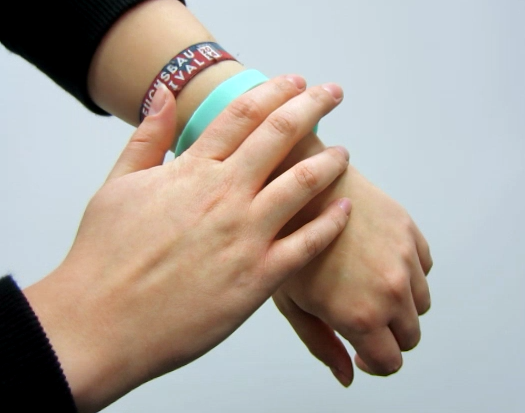
\includegraphics[width=.45\linewidth]{gfx/cover_touch.png}}
	\caption{Covering and holding the bracelet's touch surface for on/off switching or dimming}
\end{figure}

While the touch slider is covered, the hand must be held fairly steady in terms of rotation to correctly trigger the on/off function, because otherwise the dimming algorithm would trigger instead. See section \ref{sec:dimming} for a specification of the tolerated rotation when covering the touch area. If the light is switched off, the current color would be saved by the bracelet and restored on the next "on" command.

\section{Adjusting the Light Source's Brightness}
\label{sec:dimming}
Apart from switching the lights on or off, a change in brightness is the second most desired interaction in the smart lighting scenario. For example, the incentive of watching TV in the living room benefits from a dimmed light setting. However, if the user fails to locate the remote control for the television, a quick dim interaction towards brighter light facilitates the search for the missing remote control. After the item is found, the brightness level of the room's lighting can easily be dimmed back to the desired setting.

The dimming interaction is different from the other use cases, since there exists a physical solution for this task in form of dim knobs for wall outlets. Usually, those wall dimmers are rotary knobs connected to a potentiometer which dims the light source by increasing the electric resistance. Hence, the interaction of turning a knob for dimming the light level is an association for many people.

The intention was to preserve this association to make the interaction with the bracelet more intuitive. The dimming interaction is a combination of twisting the wrist while covering the bracelet's touch surface, imitating the interaction with the wall dimmer. The cover check routine is the same as described in section \ref{sec:onoff}, so covering six of the seven segments suffices to activate this function. While the touch surface is covered, the angle of the wrist rotation is constantly measured. From the way the accelerometer is mounted on the bracelet, the relevant axis for rotation is the Y-axis in the accelerometer's coordinate system. The following formula derives an angle $\alpha$ from the acceleration data \cite{Abayarjoo2013}:
\[ 
\alpha = tan^{-1}\left(\frac{y}{\sqrt{x^2 + z^2}}\right).
\]
Note that the accelerometer data must not include a gravity offset. If the observed angle exceeds certain thresholds and the current angle is at least $0.5\degree$ different from the previously measured value, a dimming step is executed and the brightness of all three color channels is reduced or increased by XX percent. A counterclockwise movement reduces the brightness, while a clockwise twist increases the brightness.

\section{Changing the Lighting Mood}
In addition to changing the brightness, the user should be able to adjust the light's color in a casual way and without thinking too much about the desired color in detail. Hence, the user is able to change the \textit{mood} of the light by touching two neighboring segments of the bracelet's touch element. Activating the left pair of segments increases the blue channel by XX percent while decreasing the red channel by YY percent; a touch on the right pair of segments causes the opposite (cf. fig. \ref{fig:mood}). Since blue colors are perceived as calming and relaxing while reds and oranges have an activating and stimulating effect \cite{Rosenstein1985}, this function can actually affect the user's mood by utilizing insights of color psychology.

\begin{figure}[bth]
	\myfloatalign
	\subfloat[Coodling down the light \textit{mood} by increasing the blue channel]
	{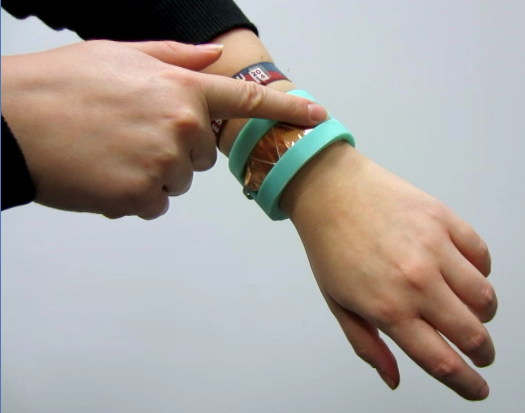
\includegraphics[width=.45\linewidth]{gfx/mood_left.png}} \quad
	\subfloat[Warming up the light \textit{mood} by increasing the red channel]
	{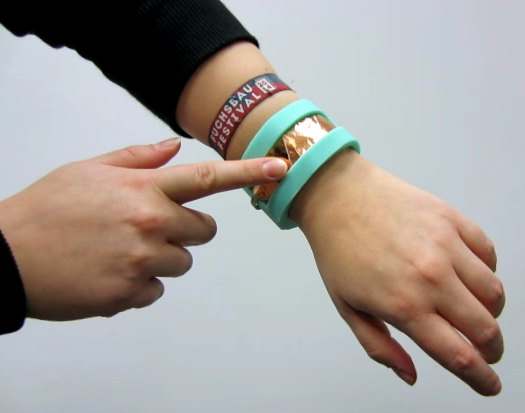
\includegraphics[width=.45\linewidth]{gfx/mood_right.png}}
	\caption{Touch interaction for \textit{mood} change}
	\label{fig:mood}
\end{figure}

\section{Precise Touch Input for Color Change}
%TODO explain rgb and hsl color ranges
Since adjusting the light color in a rather fuzzy way as described in the previous section is sometimes too imprecise, an additional function for setting the exact light color has been implemented. The RGB color model used by the lamp (cf. chapter \ref{sec:lamp}) is not very intuitive to the average user in terms of expressing a specific color in fractions of red, green and blue light, respectively, so the \ac{HSL} color model was used instead for this interaction.

\begin{figure}[bth]
	\myfloatalign
	\subfloat[The RGB color model, represented as a cube]
	{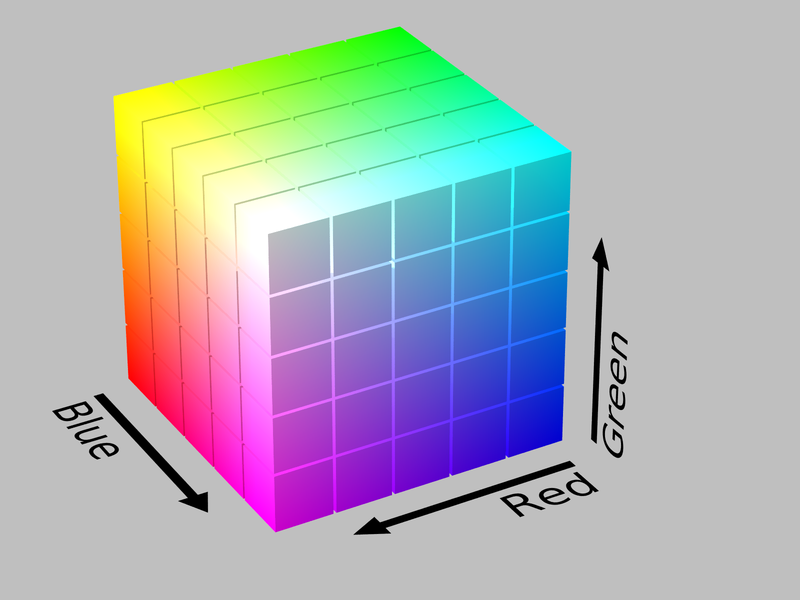
\includegraphics[width=.45\linewidth]{gfx/rgbcube.png}} \quad
	\subfloat[The \ac{HSL} color model, represented as a cylinder]
	{\label{fig:bracelet01}%
		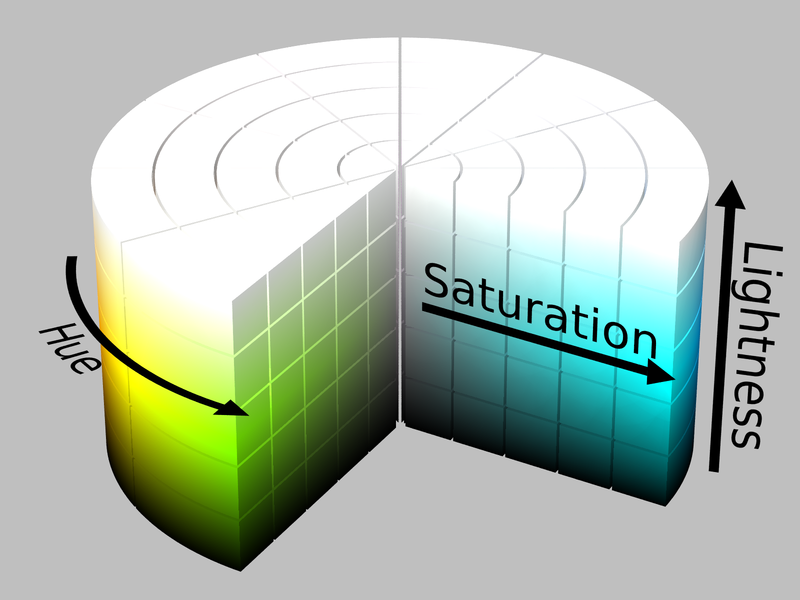
\includegraphics[width=.45\linewidth]{gfx/hslmodel.png}}
	\caption{Comparison of the RGB and \ac{HSL} color models, CC-BY-SA Michael Horvath}
\end{figure}

While the RGB color space forms a cube with red, green and blue channel on each axis, the \ac{HSL} color space forms a cylinder. Hue represents the angle, while saturation stands for the diameter and lightness for the cylinder's height. Figure \ref{fig:color} illustrates that difference. Since the conversion from \ac{HSL} to RGB color space is not trivial, a conversion algorithm had to be implemented (\cite{qwertie}, derived from \cite{graphicsgems}). For given hue $H\in \left[ 0\degree , 360\degree \right]$, saturation $S\in \left[ 0, 1\right]$ and lightness $L\in \left[ 0, 1\right]$, the chroma value $C$ is calculated first:
\[
C = \left( 1 - \left| 2L-1\right| \right) \times S
\]
An intermediate value $X$ is calculated, and, depending on the value of $H$, the values for red, green and blue can be determined.
\[
X = C\left( 1 - \frac{H}{60\degree} \mod{2} - 1\right)
\]
\[
\left(R, G, B\right) = \left(m, m, m\right) + 
\begin{cases}
(0, 0, 0) &\mbox{if } H \mbox{ is undefined} \\
(C, X, 0) &\mbox{if } 0 \leq \frac{H}{60\degree} < 1 \\
(X, C, 0) &\mbox{if } 1 \leq \frac{H}{60\degree} < 2 \\
(0, C, X) &\mbox{if } 2 \leq \frac{H}{60\degree} < 3 \\
(0, X, C) &\mbox{if } 3 \leq \frac{H}{60\degree} < 4 \\
(X, 0, C) &\mbox{if } 4 \leq \frac{H}{60\degree} < 5 \\
(C, 0, X) &\mbox{if } 5 \leq \frac{H}{60\degree} < 6
\end{cases}
\]
Where $m$ denotes a lightness offset to the color:
\[
m = L - \frac{C}{2}
\]

%TODO improve readability, explain
%\begin{lstlisting}[label=lst:hsl2rgb,language=c,frame=lt,caption=Converting from the RGB color space to the \ac{HSL} color space]
%void HSL_to_RGB(int hue, int sat, int lum, int* r, int* g, int* b){
%	int v;
%	
%	v = (lum < 128) ? (lum * (256 + sat)) >> 8 :
%	(((lum + sat) << 8) - lum * sat) >> 8;
%	if (v <= 0) {
%		*r = *g = *b = 0;
%	} else {
%		int m;
%		int sextant;
%		int fract, vsf, mid1, mid2;
%		
%		m = lum + lum - v;
%		hue *= 6;
%		sextant = hue >> 8;
%		fract = hue - (sextant << 8);
%		vsf = v * fract * (v - m) / v >> 8;
%		mid1 = m + vsf;
%		mid2 = v - vsf;
%		switch (sextant) {
%			case 0: *r = v; *g = mid1; *b = m; break;
%			case 1: *r = mid2; *g = v; *b = m; break;
%			case 2: *r = m; *g = v; *b = mid1; break;
%			case 3: *r = m; *g = mid2; *b = v; break;
%			case 4: *r = mid1; *g = m; *b = v; break;
%			case 5: *r = v; *g = m; *b = mid2; break;
%		}
%	}
%}
%\end{lstlisting}

A contact on the middle segment of the capacitive touch strip, held for approximately XX milliseconds activates this mode. The touch strip becomes a touch slider for changing the hue, while the saturation value is preset to its maximum value and lightness is set to half the maximum value. This makes the hue bright and saturated, so the user can focus on choosing the desired color. When the hue is set, a tap on the bracelet's back switches to the next component setting, namely saturation (cf. fig. \ref{fig:hslinteraction}). Tapping instead of touching somewhere on the touch surface ensures that the chosen color would not be offset by any accidental contact while trying to confirm the current selection. The bracelet's \ac{LED} acknowledges a tap with a green blink and the next parameter can be set. After setting the lightness, a tap on the backside brings the bracelet back into its standard mode, where all commands listed in this chapter are available again. During the precise color change command, the action cannot be aborted. Instead, the user needs to quickly cycle through the settings in order to leave this mode.

\begin{figure}[bth]
	\myfloatalign
	\subfloat[Activation of the color choosing mode by touching the middle segment]
	{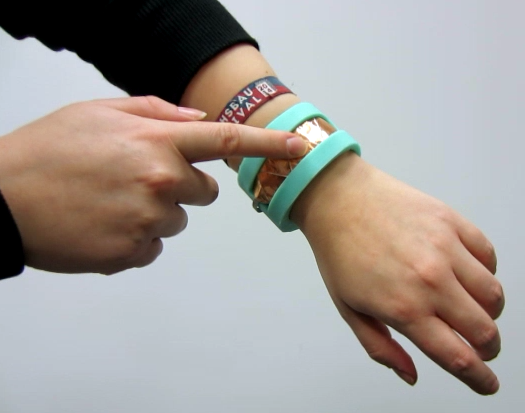
\includegraphics[width=.45\linewidth]{gfx/hsl_activation.png}} \quad
	\subfloat[Tapping on the bracelet's back side to switch to the next parameter]
	{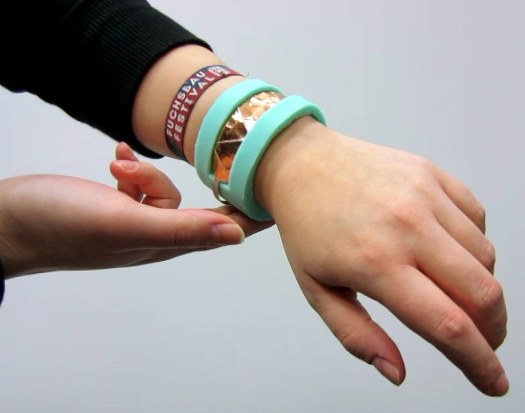
\includegraphics[width=.45\linewidth]{gfx/tap.png}}
	\label{fig:hslinteraction}
	\caption{Interaction with the bracelet to precisely set the color}
\end{figure}

\section{Template picking by Gesture Recognition}
The last form of interaction with the bracelet is by drawing gestures in the air to trigger preset color and brightness configurations. A "Z"-shaped gesture changes to a bright white light which is ideal for working, e.g. while preparing a meal in the kitchen or cleaning the house. The second gesture is a circle drawn in the air, which switches to a soft, warm-colored and slightly dimmed setting which is suitable for relaxing activities like reading or watching TV. The third gesture is a pigtail-like looping which triggers a colorful, dark purple, lounge-like setting. The gestures are depicted in \ref{fig:gestures} and the exact values for the red, green and blue channels of the lamp are listed in table \ref{tab:colors}.

\begin{table}
	\myfloatalign
	\begin{tabularx}{.8\textwidth}{ccccc}
		\toprule
		\tableheadline{Gesture} & \tableheadline{Association} & \tableheadline{Red} & \tableheadline{Green} & \tableheadline{Blue}\\ 
		\midrule
		Z & Work & $ 255 $ & $ 255 $ & $ 255 $\\
		Circle & Relax & ??? & ??? & ???\\
		Pigtail & Lounge & ??? & ??? & ???\\
		\bottomrule
	\end{tabularx}
	\caption[Color presets for gesture activation]{Color presets and associations for gesture activation}  \label{tab:colors}
\end{table}

These gestures are recorded by the bracelet's accelerometer and processed using the ``3\$ Gesture Recognizer'' \cite{Kratz2010}, an extension of the popular ``1\$ Recognizer'' by Wobbrock et. al \cite{Wobbrock2007}. The algorithm is explained in detail in the following paragraphs.

Gesture recognition is triggered by double tapping on the bracelet's back side (for a more detailed specification of the tap recognition, see section \ref{sec:config}). This focused activation was chosen to prevent accidental triggering of the gesture recognition procedure while gesturing heavily, e.g. during a conversation. A little more effort in starting this rather rarely used feature is preferred over a higher false positive rate in gesture recognition triggering. After a double tap was detected, the \ac{LED} indicates with a red glow that acceleration data is recorded while the next $150$ samples are saved for the gesture recognition algorithm.

Wobbrock as well as Kratz start their processing with a resampling step to compensate for different speeds in drawing the gesture. If the gesture was drawn quickly, it would have less samples and thus less points compared to a slowly drawn gesture. In order to be able to compare these two gestures, a resampling is performed before further processing. Therefore, the gesture is resampled to a sixed number of points before other processing takes place. Since the implementation in this thesis always records a fixed number of samples, this step is omitted. This can lead to cut off gestures when drawn too slowly or added noise at the end of a data set if the gesture was drawn too quickly. While recording test samples with various people, the record period however seemed appropriate for most gestures that were executed.

%After a gesture is recorded, it is resampled to a fixed number of points. If the gesture was drawn quickly, it would have less samples and thus less points compared to a slowly drawn gesture. In order to be able to compare these two gestures, a resampling is performed before further processing. The length of the gesture path $M$ is calculated and an increment size $I$ derived by dividing $M$ by $(N/1)$, where $N$ is the desired number of samples. The gesture path is stepped trough and after each distance $I$, a new point is inserted using linear interpolation (cf. listing \ref{lst:resample}). %TODOwe have fixed # of samples. is this necessary?

%\begin{lstlisting}[label=lst:resample,language=python,frame=lt,caption=Resampling of a points path into N evenly spaced points]
%def resample(points, N):
%	I = path_length(points) / (N - 1)
%	D = 0
%	newpoints = points[:1]
%	for i in range(1, len(points)):
%		dist = distance(points[i-1], points[i])
%		if(D + dist) > I:
%			q = points[i-1] + ((I - D)/dist) * (points[i] - points[i-1])
%			newpoints.append(q)
%			D = distance(q, points[i])
%		else:
%			D = D + dist
%	if(D + dist) > increment: #append last point manually
%		q = newpoints[-1] + ((increment - D) / dist) * (points[i] - newpoints[-1])
%		newpoints.append(q)
%	return newpoints
%\end{lstlisting}

In the next step, the gesture is prepared for matching against the templates by rotating it to a specific position. The so called \textit{indicative angle} $\theta$ between the gesture's centroid $C$ and its first point of the data set is calculated using the normalized scalar product of the centroid and the first point's position vectors. Afterwards the gesture is rotated so that $\theta$ is at $0\degree$. Wobbrock et. al. do this by using the inverse tangents function, however this is not possible in 3D space. Hence, \textit{Rodrigues' rotation formula} (named after French mathematician Olinde Rodrigues) was implemented instead. This efficient algorithm for rotating a vector in $\mathbb{R}^3$ takes the rotation angle $\theta$ as well as the axis unit vector $k$ as input, and calculates the following formula:

\begin{center}
\(
v_{rot} = v \cos\theta + (k \times v)\sin\theta + k (k \cdot v) (1 - \cos\theta).
\) \cite{koks2006}
\end{center}

After applying this function on the gesture, a good starting point is created for the actual recognizing part of the algorithm. Listing \ref{lst:rotate2zero} illustrates the rotation procedure.

\begin{lstlisting}[label=lst:rotate2zero,language=python,frame=lt,caption=Rotation of points so that their indicative angle is at $0 \degree$]
def rotate_to_zero(points):
	c = centroid(points)
	theta = acos(points[0] * c / (|points[0]| * |c|)
	newpoints = rotate_by(points, -theta)
	return newpoints
\end{lstlisting}

In order to harmonize gestures of different sizes which represent slow or quick movements, the points are scaled to a reference cube with edge length of $100$ units and translated so that the respective centroid $C$ is on the origin (cf. listing \ref{lst:scale+translate}).

\begin{lstlisting}[label=lst:scale+translate,language=python,frame=lt,caption=Scaling to reference cube and translation to origin]
def scale_and_translate(points, size): # size=100
	B = Bounding_Box(points)
	newpoints = []
	for p in points:
		q = Point()
		q.x = (p.x * (size / B.width)) - c.x
		q.y = (p.y * (size / B.height)) - c.y
		q.z = (p.z * (size / B.depth)) - c.z
		newpoints.append(q)
	return newpoints
\end{lstlisting}

After these harmonization and preparation steps, the gestures are matched against the prerecorded templates (cf. listing \ref{lst:recognize}). The aforementioned steps are applied to templates as well as to newly recorded gestures, the following algorithms only apply to unrecognized gestures.

\begin{lstlisting}[label=lst:recognize,language=python,frame=lt,caption=Matching candidate gesture against every template]
def recognize(points, templates, rescale_size):
	theta_min = -180
	theta_max = 180
	theta_delta = 2

	best = float("inf")
	for t in templates:
		dist = distance_at_best_angle(points, t, theta_min, theta_max, theta_delta)
		if dist < best:
			best = dist
			t_best = t
	return t_best
\end{lstlisting}

The candidate is compared to all stored templates using the average \ac{MSE} as a scoring metric. The optimal position between the candidate gesture and a stored template is possibly offset by a certain rotation, so the optimal combination of angles between the two gestures needs to be determined. Since rotations are costly in terms od computation time, the candidate gesture should be aligned to the template in as few tries as possible. Hence, as proposed by \cite{Kratz2010}, a \ac{GSS} is used to find the optimal angles $\alpha$, $\beta$, and $\gamma$ for rotation around the three axis of the coordinate system.

The \ac{GSS} algorithm was invented by US-American statistician Jack Kiefer in 1953  and is conceptualized to find the minimum value $x^*$ of a unimodal function $f\left(x\right)$ in a given interval $\left[a,b\right]$ \cite{Kiefer1953}. Two function points $f(x_1)$ and $f(x_2)$ with 
\[ x_1=a+\left(1-\phi\right)\left(b-a\right) \\
x_2=a+\phi\left(b-a\right) \]
are calculated and compared, where 
\[\phi=\frac{2}{\left(1+\sqrt{5}\right)}\]
denotes the Golden Section constant. If $f\left(x_1\right) < f\left(x_2\right)$, the interval for the next iteration becomes $\left[a,x_1\right]$ and the new test points are calculated as described above with respect to the new interval borders. Note that the value $f\left(x_1\right)$ can be reused \cite{chang2009n}. If $f\left(x_1\right) > f\left(x_2\right)$, the interval for the next iteration step changes to $\left[x_2, b\right]$ respectively. If the function points differ not more than a given $x_\Delta$, the current minimum will be accepted as the algorithm's result.

In the context of the implemented gesture recognizer, the function to be minimized is the distance between a gesture candidate and a certain template at the best angle. Since the recognizer works with three-dimensional data, there is not a single angle for rotation, but one for each coordinate axis. Hence, the \ac{GSS} needs to be adapted for three dimensions.

As listing \ref{lst:daba} illustrates, the three-dimensional approach is similar to the one-dimensional algorithm. Each of the variables $\alpha$, $\beta$, $\gamma$ has its own search interval and a pair of calculated values. This leads to eight function points to be evaluated in each iteration, denoted in the code by variables \texttt{f1} to \texttt{f8}. The minimum of these values is calculated and the intervals adjusted accordingly. Note that in every case one function value from the previous step can be carried over, for example when \texttt{f1} is the minimum, its value is used for the new \texttt{f8}.

\begin{lstlisting}[label=lst:daba,language=python,frame=lt,caption=Three-dimensional Golden Section Search for finding the best angle between a candidate gesture and a template]
def distance_at_best_angle(p, t, theta_min, theta_max, theta_delta):
	phi = 0.5 * (-1 + math.sqrt(5))
	a_min = theta_min
	a_max = theta_max
	b_min = theta_min
	b_max = theta_max
	g_min = theta_min
	g_max = theta_max

	x1 = phi * a_min + (1 - phi) * a_max
	x2 = (1 - phi) * a_min + phi * a_max
	y1 = phi * b_min + (1 - phi) * b_max
	y2 = (1 - phi) * b_min + phi * b_max
	z1 = phi * g_min + (1 - phi) * g_max
	z2 = (1 - phi) * g_min + phi * g_max	

	f1 = distance_at_angle(p, t, x1, y1, z1)
	f2 = distance_at_angle(p, t, x1, y1, z2)
	f3 = distance_at_angle(p, t, x1, y2, z1)
	f4 = distance_at_angle(p, t, x1, y2, z2)
	f5 = distance_at_angle(p, t, x2, y1, z1)
	f6 = distance_at_angle(p, t, x2, y1, z2)
	f7 = distance_at_angle(p, t, x2, y2, z1)
	f8 = distance_at_angle(p, t, x2, y2, z2)

	while (|a_max - a_min| > theta_delta) or (|b_max - b_min| > theta_delta) or (|g_max - g_min| > theta_delta):	
		min_f = min(f1, f2, f3, f4, f5, f6, f7, f8)
		if min_f == f1: #x1, y1, z1
			a_max = x2
			x2 = x1
			x1 = phi * a_min + (1 - phi) * a_max
			b_max = y2
			y2 = y1
			y1 = phi * b_min + (1 - phi) * b_max
			g_max = z2
			z2 = z1
			z1 = phi * g_min + (1 - phi) * g_max
			f8 = f1
			f1 = distance_at_angle(p, t, x1, y1, z1)
			...
			f7 = distance_at_angle(p, t, x2, y2, z1)
		elif min_f == f2: #x1, y1, z2
			...
		else: #x2, y2, z2
			...
	return min(f1, f2, f3, f4, f5, f6, f7, f8)
\end{lstlisting}

To determine the distance between a gesture and a certain template at given angles $\alpha$, $\beta$, and $\gamma$, the gesture is rotated using the Rodrigues rotation formula discussed in the context of the indicative angle above. The rotation formula needs an axis and an angle for executing the rotation, but the \ac{GSS} works with three angles. Therefore, the rotation matrix formed by the angles needs to be transformed into a Euler axis and angle pair for use in the implemented rotation formula. The authors of \cite{Kratz2010} state the following rotation matrix in their reference implementation \cite{repo:3dollar}:
%TODO explain euler axis/angle?
\[
A = 
\begin{pmatrix}
\cos{\alpha}\cos{\beta} & \cos{\alpha}\sin{\beta}\sin{\gamma} - \sin{\alpha}\cos{\gamma} & \cos{\alpha}\sin{\beta}\cos{\gamma} + \sin{\alpha}\sin{\gamma} \\
\sin{\alpha}\cos{\beta} & \sin{\alpha}\sin{\beta}\sin{\gamma} + \cos{\alpha}\cos{\gamma} & \sin{\alpha}\sin{\beta}\cos{\gamma} - \cos{\alpha}\sin{\gamma} \\
-\sin{\beta} & \cos{\beta}\sin{\gamma} & \cos{\beta}\cos{\gamma}
\end{pmatrix}
\]

The Euler rotation angle $ \theta $ is composed by the matrix's diagonal elements.
\begin{eqnarray*}
\theta & = & \arccos\left(\frac{1}{2}\left(A_{11} + A_{22} + A_{33} - 1\right)\right) \\
       & = & \arccos\left(\frac{1}{2}\left(\cos\alpha\cos\beta+\sin\alpha\sin\beta\sin\gamma+\cos\alpha\cos\gamma+\cos\beta\cos\gamma-1\right)\right)
\end{eqnarray*}
The rotation axis vector $ e $ can be derived from $ A $ and $ \theta $ as follows:
\begin{eqnarray*}
e_1 & = &  \frac{A_{32} - A_{23}}{2\sin\theta} \\
    & = & \frac{\sin\alpha\sin\beta\cos\gamma-\cos\alpha\sin\gamma-\cos\beta\sin\gamma}{2\sin\theta} \\
e_2 & = & \frac{A_{13} - A_{31}}{2\sin\theta} \\
    & = & \frac{-\sin\beta-\cos\alpha\sin\beta\cos\gamma-\sin\alpha\sin\gamma}{2\sin\theta} \\
e_3 & = & \frac{A_{21} - A_{12}}{2\sin\theta} \\
    & = & \frac{\cos\alpha\sin\beta\sin\gamma-\sin\alpha\cos\gamma-\sin\alpha\cos\beta}{2\sin\theta}
\end{eqnarray*}

And like this, the angles determined in algorithm \ref{lst:daba} lead to an axis/angle rotation which is performed on the candidate gesture.

Once the best template for a candidate gesture is found, the corresponding index in the stored template list is returned and the recognized gesture triggers certain changes in the light source's color or brightness. Note that this gesture recognition algorithm is only used for recognition of the preset gestures formulated at the beginning of this section.


\section{Presets and Configuration}
\label{sec:config}
Gesture recording and recognition is triggered by a gentle double tap on the bracelet. This small but focused activation reduces unwanted triggering of the gesture recognition process, e.g. while gesturing heavily, and thus reducing false positives. The tap detection functionality is a built-in feature of the bracelet's accelerometer, configuration parameters for this process are listed in table \ref{tab:tapconf}.

In order to be recognized as a tap interaction, the initial impulse needs to be at least XX g in intensity. When calibrated like this, jerky movements like suddenly raising the hand at a high speed are correctly not recognized as a tap. However since the threshold is that high, the activation tap needs to be executed directly on the hardware which is located on the inner wrist.

The \texttt{PULSE\_TMLT} register configures the maximum time interval between the  impulse exceeding the threshold on the Z axis and falling back under said threshold. If the mentioned interval lasts at most $6.25 ms$, the interaction is considered as a tap.

After a tap is detected, all impulses in the following $25ms$ are ignored by the detection mechanism. This prevents bouncing effects and detecting multiple taps in a singe tap movement.

The MMA8652FC accelerometer is able to distinguish between single and double taps. The last configuration register listed in table \ref{tab:tapconf} is a parameter for double tap detection. It specifies the maximum time interval between two double taps and is set to $500 ms$, the same time interval as the Microsoft Windows default between two mouse clicks of a double click \cite{doubleclick}.

\begin{table}
	\myfloatalign
	\begin{tabularx}{\textwidth}{lll} \toprule
		\tableheadline{Register Name} & \tableheadline{Parameter} & \tableheadline{Value}\\ 
		\midrule
		\texttt{PULSE\_THSZ} & Tap Detection Threshold & $100 g$\\ %TODO on +/-8g scale @.063g/LSB
		\texttt{PULSE\_TMLT }& Interval between Start and End Pulse & $6.25 ms$\\
		\texttt{PULSE\_LTCY} & Ignore Interval after Detection & $25 ms$\\
		\texttt{PULSE\_WIND} & Maximum Double Tap Interval & $500ms$ \\
		\bottomrule
	\end{tabularx}
	\caption[Tap detection configuration]{Single- and double tap detection configuration for the MMA8652FC digital accelerometer}  \label{tab:tapconf}
\end{table}

Apart from accelerometer calibration, the gesture recognition algorithms needs template gestures, against which the interactively recorded data is matched. Wobbrock et. al. as well as Kratzand Rohs most likely use artificially constructed templates, though neither of them explicitly states this in their work \cite{Wobbrock2007} \cite{Kratz2010}. Constructing artificial templates for 2D stylus-based input is very easy, since the stylus produces a series of lines, rather independently from the used speed or size. When working with accelerometer data however, the recorded data is more heterogeneous, since quickly drawn gestures result in higher amplitudes in the raw data. Since it is very difficult to find the right speed and size to artificially construct template gestures, an empirical approach was used.

Ten gesture executions of each type (Z, circle, and pigtail) were recorded by eight people. Then, one gesture after another was probed as a template and statistics for correct matches as well as false positive matches were recorded. Since gestures with the least false positive rate also share very low matching rates, a ratio of
\[
\frac{\text{\# correct matches}}{\text{\# false positives}}
\]
was calculated to determine the most representative gestures. The best N gestures according to said metric were chosen as templates for the live gesture detection.